\section{Architectural styles}  

\begin{definition}
    An \emph{architectural style} determines the vocabulary of components and connectors that can be used in instances of that style, together with a set of constraints on how they can be combined.
    These can include topological constraints on architectural descriptions (e.g., no cycles). 
    Other constraints—say, having to do with execution semantics—might also be part of the style definition.
\end{definition}

\subsection*{Client-server}
The client-server architectural style is primarily employed in distributed applications, where the client initiates requests, and the server delivers responses.
\begin{figure}[H]
    \centering
    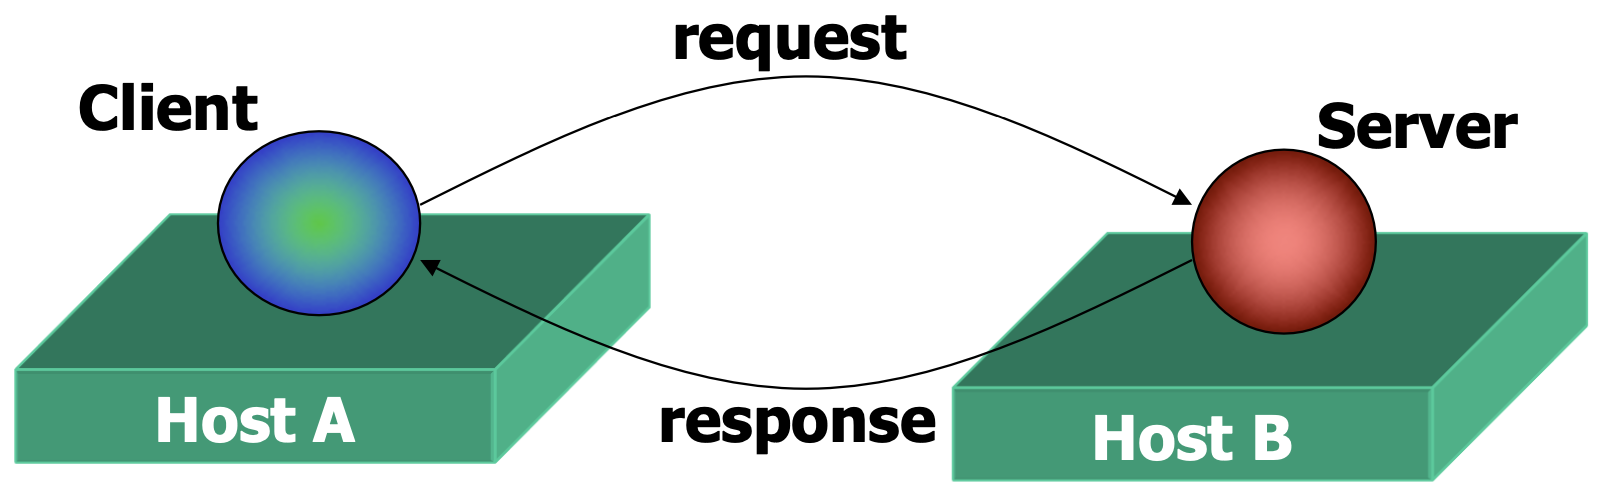
\includegraphics[width=0.5\linewidth]{images/clientserver.png}
    \caption{Client-server architecture general schema}
\end{figure}
This approach proves beneficial in situations where multiple users require access to a common resource, when there is a need to remotely access existing software, and when it is advantageous to structure the system around a shared functionality that multiple components utilize.
Key technical considerations for this architectural style include the design and documentation of well-defined interfaces for the server and the need to ensure the server's capability to handle concurrent requests efficiently.